\section{Creation of the dataset}
\label{sec:creation-dataset}
This research investigates how agents use referring expressions to discriminate objects seen in images based on their relations.
For that reason, the original CLEVR framework offers too little control over how a new dataset is created.
Especially, which objects and in which attributes they share with each other in each image can't be controlled.
Following, we extended the framework for generating new datasets.\footnote{\href{https://github.com/DominikKuenkele/MLT\_Master-Thesis\_clevr-dataset-gen}{https://github.com/DominikKuenkele/MLT\_Master-Thesis\_clevr-dataset-gen}}
By this, the objects in the generated images are controlled to have different human-recognizable attributes, namely the \emph{shape}, \emph{size} and \emph{color}.
These attributes also correspond to referring expressions in natural language such as English.
% To simplify the generation and the succeeding training of the models, we only focused on the attributes with a high impact on the appearance of the object, namely the \emph{shape}, \emph{size} and \emph{color}.
The \emph{material} is always the same for all objects in a generated image.
There were three main extensions to the framework:
% SD: Too informal
% SD: We create a new dataset based on the CLEVR framework where we control the appearance of scenes in a referring expression task.
% SD: The scenes are controlled by human-recognisable attributes of object such as object shape, colour and type. These attributes also correspond to referring expressions in natural language such as English.
% SD: We create two contexts of scenes, one with two objects and one with five. 
% SD: We also control for the number of attributes shared between the target and the distractor.
% DK: creation of dataset later (here only the general rules), (added; done)

First, objects in the scene were separated into three categories: one \emph{target object}, objects in a \emph{target group} and \emph{distractor} objects.
The target object is the main object in the scene and the models are trained to identify and communicate between each other.
All other objects and their relations are based on this target object.
The target group contains similar objects to the target object.
These are objects that the agents need to discriminate the target object from.
Finally, the distractors are objects that add noise to the scene and should make it more complex. They are expected to teach the agents more precise descriptions of the target object.
The number of the objects in both groups can be controlled.

In a second step, when generating the images it is possible to define the relations between \emph{target object}/\emph{target group} and \emph{target object}/\emph{distractors}.
The relation is defined as \textbf{how many} attributes of the target object are identical with the attributes of a single object in the target group and distractors respectively.
For example the target object is a \emph{small red cube}.
If two attributes are shared between target object and target group, objects in the target group could include \emph{small blue cube}, \emph{big red cube} or \emph{small red sphere}, but couldn't include another \emph{small red cube} or a \emph{small blue cylinder}.
The number of shared attributes can also be set to a range to control how challenging the referring task is.
% SD: To control how challenging the referring task is
% DK: (done)

Lastly, it is also possible to define exactly \textbf{which} attributes should be shared between the target object and the groups.
For example, it can be defined to have the same size for objects in the target group, but have different, randomly selected shapes and colors.
This allows for a very controlled generation of relations between the objects in the scene.
% SD: Introduce other images earlier?
% DK: I think 'Dale-5' is the most interesting image to make the point here. The others are introduced later, in the order of the pictures. So I don't think I also can change the order the pictures. (done)
Figure \ref{fig:clevr-dale-5} shows one generated image with this extended source code.
Here, the target object is the large purple cylinder.
The target group contains four objects that share zero to a maximum of two attributes.
It is not controlled, which attributes are shared (they are selected randomly). The large purple cylinder shares the same color and size with the large purple sphere, the same size with both cubes and no attribute with the small turquoise sphere.
There are no distractor objects.
% SD: It depends what you mean by distractor objects. I’d say they are all distractor objects by the virtue they share attributes. The system has to learn understanding of an intersection of these attributes.
% DK: I refer to the definitions in the paragraphs above, namley target object, target groub and distrctors. (done)

For all generated datasets in the following sections, the general constraints and settings are as close as possible to the original CLEVR dataset.
The size of the generated images is 480x320 pixels.
10.000 images are created for each of the datasets.
Each image contains a maximum of 10 objects, that are not intersecting, have the same minimum distance between objects and are at least partially visible from the camera.
% SD: Note that since objects are generated as a part of 3-d scenes, they may appear differently on images: size, occlusion, shading, rotation. We also expect the model to learn from this noise and which therefore makes the task much harder and a task that approximates natural environment compared to the task where we would use abstract geometric shapes projected on a 2-d plane.
% DK: added in the general description of CLEVR since it is not my extention (done)
% TODO: we create the follwoing dataset ....

\begin{figure}[ht]
    \centering
    \subfigure['CLEVR single', \emph{large yellow sphere}]{
        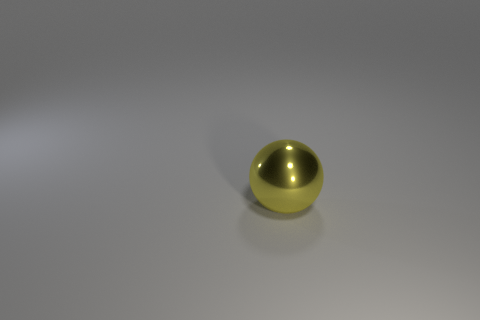
\includegraphics[width=0.43\linewidth]{figures/CLEVR_single.png}
        \label{fig:clevr-single}
    }
    \subfigure['CLEVR color', \emph{small brown cylinder}]{
        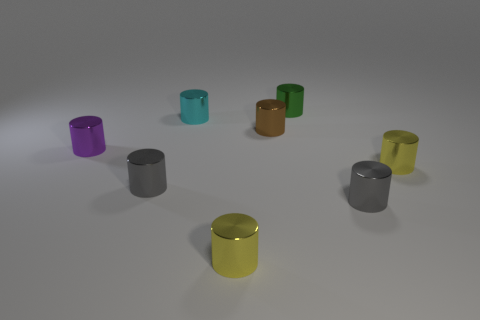
\includegraphics[width=0.43\linewidth]{figures/CLEVR_color.png}
        \label{fig:clevr-color}
    }
    \subfigure['Dale-2', \emph{small green cylinder}]{
        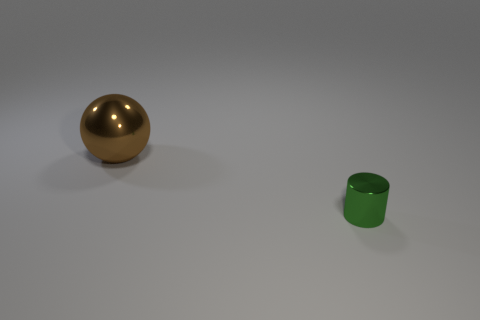
\includegraphics[width=0.43\linewidth]{figures/CLEVR_dale-2.png}
        \label{fig:clevr-dale-2}
    }
    \subfigure['Dale-5', \emph{large purple cylinder}]{
        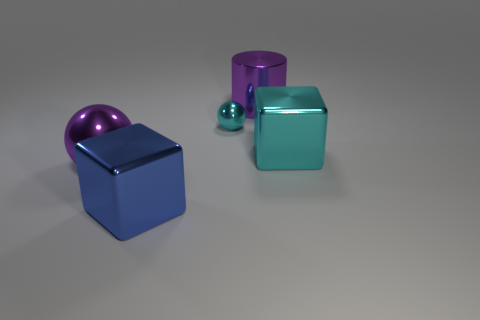
\includegraphics[width=0.43\linewidth]{figures/CLEVR_dale-5.png}
        \label{fig:clevr-dale-5}
    }
    \caption{Example images of each dataset, with the target object specified}
    \label{fig:clevr-examples}
\end{figure}

\subsection{CLEVR single}
The simplest new dataset is called 'CLEVR single'.
This is a very simple dataset and has the purpose to simplify the problem the model needs to learn as much as possible.
Each scene in the dataset contains only one single object, the target object.
There are neither objects in the target nor in the distractor group.
All attributes are assigned randomly to the target object.
The differences across the whole dataset are the locations and rotations of the objects.
With this dataset, neural models can focus on only the features, as well as the locations of this single object.
There are no objects that distract the model from extracting features from the target object.
This helps to understand if the models are actually able to assign features or learn locations of these features in an image.
Figure \ref{fig:clevr-single} shows an example with the only object being the \emph{large yellow sphere}.

\subsection{CLEVR color}
The second dataset that is created is called 'CLEVR color'.
The purpose of this dataset is to create scenes, where the target object is completely unique and as easily identifiable as possible.
For this reason, there exist only two groups in the scene, the target object and distractors.
The distractor group can contain in between 6 and 9 objects.
To make the discrimination as simple as possible the target object and the objects in the target group share exactly two attributes.
% SD: Wouldn’t it make sense to introduce the discussion of how scenes can be generated with attributes somewhere here? Again, I felt we were projecting forward earlier without understanding the task.
% DK: before, I only wanted to outlie the rules for the creation, i.e. what is possible with it. Since the code to create the datasets is also a contribution, I wanted to let it stand on its own. Here I only describe how these rules are applied for each new dataset. (QUESTION)
Furthermore, to simplify the relation between target object and distractors over the whole dataset, it is also controlled which attributes are shared.
The distractors have always the same size and shape as the target object, but the color is different.
The reason for choosing the color as the only discriminating attribute is that it is assumed that the color is easier to learn for neural models as opposed to for instance abstract shapes.
% SD: But why not test the limits and the harder examples?
% DK: In the experiments, the models often hda problems to learn anything (with the complex dataset), which is why I reduced the complexity with the 'color' dataset. (done)


As seen in Figure \ref{fig:clevr-color}, the \emph{small brown cylinder} is unique.
By this, it is possible to refer to the target object using the attributes with four different combinations: the \emph{brown} object, the \emph{brown cylinder}, the \emph{small brown} object and the \emph{small brown cylinder}.
All attributes, apart from the color are not discriminating the target object from the distractors.
Notice as well that this restriction doesn't apply to the distractors, where multiple objects with the same color are allowed.
In other words, the choice of attributes is random for the distractors, and they may overlap.
% SD: In order words, the choice of attributes is random for distractor and there may be an overlap between the same distractor objects. This is because we do not control overlap attributes over distractor, I.e. random.
% DK: (added; done)

\subsection{CLEVR Dale datasets}
% SD: In the previous dataset the target and distractor are discriminated by ONE attribute exactly.
% DK: TODO
The above described dataset is very restrictive in the relation between the objects, where only \emph{one} attribute is used to disambiguate them.
The number and the type of shared attributes are controlled exactly.
In the real world, objects have overlapping attributes and hence objects can only be identified by an intersection of multiple attributes.
In real situations, there is no restriction at all how objects or things relate to each other.
Natural language emerged that can refer to distinct attributes of these objects to discriminate them from each other.
This emergence of referring attributes and their combination is studied deeper in this work.
% SD: In real world, objects have over-lapping attributes and hence a single object can only be identified by an intersection of attributes.
% DK: (rephrased; done)

% SD: However, we do not do this randomly but ge5 inspiration from the Dale and Reiter generation algorithm who observe that attributes in descriptions occur in certain order and are added incrementally in a certain hierarchy. This way we approximate the information in the scenes to human cognition and we hope that the system will be able to exploit that (we would really need to study and compare it with another dataset where attributes are add3d randomly to confirm that there is an effect of h7man. Ignition).
% DK: see below (done)
For this, we created a dataset that allows almost any relation between a target object and the distractors.
However, the creation is inspired by incremental algorithm for the Generation of Referring Expressions (GRE) described in \citep{Dale1995} who observe that attributes in descriptions occur in certain order and are added incrementally in a certain hierarchy.
This algorithm ensures that every scene contains a unique object in respect to its and the distractors' attributes.
Using the algorithm, one can refer to an object using its attributes to discriminate it from all other objects as efficiently as possible.
In other words, the object is described unambiguously using the lowest number of words.
For the dataset that means that zero, one or two attributes can be shared between the target object and distractor objects.
This ensures the uniqueness of the target object.
On the other side, it is not controlled which attributes are shared.
% SD: The sharing of attributes should be according to the Dale and Reiter hierarchy, shouldn’t it? Two attributes, big blue (cube|sphere)
% DK: During the creation of the dataset, only the number of shared attributes is shared that we get different numbers of overlaps. Only the captions (that are created later and used as input or output for some models/agents) rely directly on the algorithm. At this point, I only wanted to bring up the reason for this, which is the usage of the algorithm in human referring expressions and how it compares to machine referring expressions. (done)
These are assigned randomly.
There is again no control over the relations between distractors, which means that distractors can appear multiple times.

Two datasets following these rules are created.
The Dale-2 dataset contains one target object and one distractor (see Figure \ref{fig:clevr-dale-2}), while the Dale-5 dataset contains one target object and exactly four distractors.
Consider Figure \ref{fig:clevr-dale-5}, with the target object being the \emph{large purple cylinder}. The large purple sphere shares the size and color, the two cubes only share the size, and the small turquoise sphere doesn't share any attribute.
% SD: It’s actually the reverse in which descriptions are generated, we start left to right: large purple (are shared), the last attribute must thus be unique. Generation proceeds in the opposite order, one would just say sphere. We should clarify this. Now it is very hard to understand.
% DK: That's true for the generation of the descriptions. This is explained in chapter 4.2.1 where the captions are needed for the training as input. As said before, the algorithm was not directly used and is just the reason. (done)

These two datasets allow a more realistic look in how models can acquire knowledge about attributes of objects.
More specifically it helps to understand how models learn to discriminate objects from each other, since the model may only need to learn discriminative features of objects and not all features of the whole object.

\cmtDK{probabilities of shared attributes for both Dale-2 and Dale-5}